% GNUPLOT: LaTeX picture with Postscript
\begingroup
\newcommand{\ft}[0]{\footnotesize}
  \makeatletter
  \providecommand\color[2][]{%
    \GenericError{(gnuplot) \space\space\space\@spaces}{%
      Package color not loaded in conjunction with
      terminal option `colourtext'%
    }{See the gnuplot documentation for explanation.%
    }{Either use 'blacktext' in gnuplot or load the package
      color.sty in LaTeX.}%
    \renewcommand\color[2][]{}%
  }%
  \providecommand\includegraphics[2][]{%
    \GenericError{(gnuplot) \space\space\space\@spaces}{%
      Package graphicx or graphics not loaded%
    }{See the gnuplot documentation for explanation.%
    }{The gnuplot epslatex terminal needs graphicx.sty or graphics.sty.}%
    \renewcommand\includegraphics[2][]{}%
  }%
  \providecommand\rotatebox[2]{#2}%
  \@ifundefined{ifGPcolor}{%
    \newif\ifGPcolor
    \GPcolortrue
  }{}%
  \@ifundefined{ifGPblacktext}{%
    \newif\ifGPblacktext
    \GPblacktextfalse
  }{}%
  % define a \g@addto@macro without @ in the name:
  \let\gplgaddtomacro\g@addto@macro
  % define empty templates for all commands taking text:
  \gdef\gplbacktext{}%
  \gdef\gplfronttext{}%
  \makeatother
  \ifGPblacktext
    % no textcolor at all
    \def\colorrgb#1{}%
    \def\colorgray#1{}%
  \else
    % gray or color?
    \ifGPcolor
      \def\colorrgb#1{\color[rgb]{#1}}%
      \def\colorgray#1{\color[gray]{#1}}%
      \expandafter\def\csname LTw\endcsname{\color{white}}%
      \expandafter\def\csname LTb\endcsname{\color{black}}%
      \expandafter\def\csname LTa\endcsname{\color{black}}%
      \expandafter\def\csname LT0\endcsname{\color[rgb]{1,0,0}}%
      \expandafter\def\csname LT1\endcsname{\color[rgb]{0,1,0}}%
      \expandafter\def\csname LT2\endcsname{\color[rgb]{0,0,1}}%
      \expandafter\def\csname LT3\endcsname{\color[rgb]{1,0,1}}%
      \expandafter\def\csname LT4\endcsname{\color[rgb]{0,1,1}}%
      \expandafter\def\csname LT5\endcsname{\color[rgb]{1,1,0}}%
      \expandafter\def\csname LT6\endcsname{\color[rgb]{0,0,0}}%
      \expandafter\def\csname LT7\endcsname{\color[rgb]{1,0.3,0}}%
      \expandafter\def\csname LT8\endcsname{\color[rgb]{0.5,0.5,0.5}}%
    \else
      % gray
      \def\colorrgb#1{\color{black}}%
      \def\colorgray#1{\color[gray]{#1}}%
      \expandafter\def\csname LTw\endcsname{\color{white}}%
      \expandafter\def\csname LTb\endcsname{\color{black}}%
      \expandafter\def\csname LTa\endcsname{\color{black}}%
      \expandafter\def\csname LT0\endcsname{\color{black}}%
      \expandafter\def\csname LT1\endcsname{\color{black}}%
      \expandafter\def\csname LT2\endcsname{\color{black}}%
      \expandafter\def\csname LT3\endcsname{\color{black}}%
      \expandafter\def\csname LT4\endcsname{\color{black}}%
      \expandafter\def\csname LT5\endcsname{\color{black}}%
      \expandafter\def\csname LT6\endcsname{\color{black}}%
      \expandafter\def\csname LT7\endcsname{\color{black}}%
      \expandafter\def\csname LT8\endcsname{\color{black}}%
    \fi
  \fi
  \setlength{\unitlength}{0.0500bp}%
  \begin{picture}(7936.00,5668.00)%
    \gplgaddtomacro\gplbacktext{%
      \colorrgb{0.50,0.50,0.50}%
      \put(594,751){\makebox(0,0)[r]{\strut{} 0}}%
      \colorrgb{0.50,0.50,0.50}%
      \put(594,1283){\makebox(0,0)[r]{\strut{} 2}}%
      \colorrgb{0.50,0.50,0.50}%
      \put(594,1815){\makebox(0,0)[r]{\strut{} 4}}%
      \colorrgb{0.50,0.50,0.50}%
      \put(594,2347){\makebox(0,0)[r]{\strut{} 6}}%
      \colorrgb{0.50,0.50,0.50}%
      \put(594,2879){\makebox(0,0)[r]{\strut{} 8}}%
      \colorrgb{0.50,0.50,0.50}%
      \put(594,3411){\makebox(0,0)[r]{\strut{} 10}}%
      \colorrgb{0.50,0.50,0.50}%
      \put(594,3943){\makebox(0,0)[r]{\strut{} 12}}%
      \colorrgb{0.50,0.50,0.50}%
      \put(594,4475){\makebox(0,0)[r]{\strut{} 14}}%
      \colorrgb{0.50,0.50,0.50}%
      \put(594,5007){\makebox(0,0)[r]{\strut{} 16}}%
      \colorrgb{0.50,0.50,0.50}%
      \put(773,484){\makebox(0,0){\strut{}4}}%
      \colorrgb{0.50,0.50,0.50}%
      \put(907,484){\makebox(0,0){\strut{}9}}%
      \colorrgb{0.50,0.50,0.50}%
      \put(1095,484){\makebox(0,0){\strut{}16}}%
      \colorrgb{0.50,0.50,0.50}%
      \put(1337,484){\makebox(0,0){\strut{}25}}%
      \colorrgb{0.50,0.50,0.50}%
      \put(1632,484){\makebox(0,0){\strut{}36}}%
      \colorrgb{0.50,0.50,0.50}%
      \put(1981,484){\makebox(0,0){\strut{}49}}%
      \colorrgb{0.50,0.50,0.50}%
      \put(2384,484){\makebox(0,0){\strut{}64}}%
      \colorrgb{0.50,0.50,0.50}%
      \put(2840,484){\makebox(0,0){\strut{}81}}%
      \colorrgb{0.50,0.50,0.50}%
      \put(3351,484){\makebox(0,0){\strut{}100}}%
      \colorrgb{0.50,0.50,0.50}%
      \put(3914,484){\makebox(0,0){\strut{}121}}%
      \colorrgb{0.50,0.50,0.50}%
      \put(4532,484){\makebox(0,0){\strut{}144}}%
      \colorrgb{0.50,0.50,0.50}%
      \put(5203,484){\makebox(0,0){\strut{}169}}%
      \colorrgb{0.50,0.50,0.50}%
      \put(5928,484){\makebox(0,0){\strut{}196}}%
      \colorrgb{0.50,0.50,0.50}%
      \put(6707,484){\makebox(0,0){\strut{}225}}%
      \colorrgb{0.50,0.50,0.50}%
      \put(7539,484){\makebox(0,0){\strut{}256}}%
      \csname LTb\endcsname%
      \put(220,2879){\rotatebox{-270}{\makebox(0,0){\strut{}Przyspieszenie}}}%
      \put(4156,154){\makebox(0,0){\strut{}Liczba procesów}}%
      \put(4156,5337){\makebox(0,0){\strut{}Hybrydowy algorytm Cannona}}%
      \put(5928,1203){\makebox(0,0)[l]{\strut{}Algorytm naiwny}}%
    }%
    \gplgaddtomacro\gplfronttext{%
      \csname LTb\endcsname%
      \put(3149,4834){\makebox(0,0)[r]{\strut{}Cannon-OMP, 1 wątek}}%
      \csname LTb\endcsname%
      \put(3149,4614){\makebox(0,0)[r]{\strut{}Cannon-OMP, 4 wątków}}%
      \csname LTb\endcsname%
      \put(3149,4394){\makebox(0,0)[r]{\strut{}Cannon-OMP, 12 wątków}}%
      \csname LTb\endcsname%
      \put(3149,4174){\makebox(0,0)[r]{\strut{}Cannon}}%
    }%
    \gplbacktext
    \put(0,0){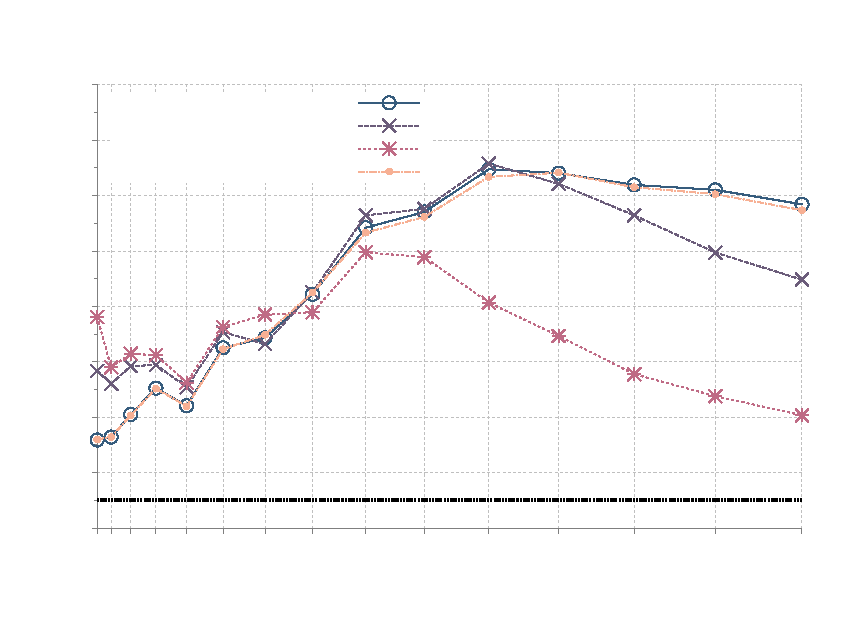
\includegraphics{scal_cannon_omp}}%
    \gplfronttext
  \end{picture}%
\endgroup
